\section{Introduction}
Education buildings are common examples of commercial buildings that involve a
meeting of a large number of people withing a closed area.
While designing such types of buildings, a common goal is to maximize the
productivity of the available space, but it is essential to consider the
safety aspects as well.
One of such aspects is how efficiently can emergency evacuations be carried out
due to the threat of fire.
Whether a building layout is suitable for emergency evacuation is a difficult
and rather ambiguous decision due to the fact that numerous factors must be
taken into account, such as fire and smoke spreading, behaviour of every single
individual as well as crowd dynamics and other random events.
Modelling [ims-8] such situations can give an insight into the safety aspects
of a building and identify its flaws.

This project addresses a question of how such evacuation processes can be
modelled using cellular automata [ims-316].
Our work is mainly based on a research by Tissera et al.~\cite{Tissera1};
several modifications enhancing pedestrian behaviour are introduced, some of
them inspired by the research by Yuan et al.~\cite{Yuan}.
We will use our approach to model evacuation processes inside two selected
buildings, namely, D and E wings of a FIT BUT building~\cite{FIT}.
Using these models we will simulate different fire scenarios and collect
various statistics [ims-35] in order to evaluate key safety aspects of the
systems [ims-7] under investigation.

Section 2 describes some basic concepts: a theory behind cellular automata,
the laws of fire and smoke spreading, the principles behind people movement and
consequences of a smoke poisoning.
In Section 3 we invoke these concepts and introduce an abstract model [ims-9]
of a system.
Section 4 briefly describes seletecte implementation features.

{In Section 5 TODO}

\section{Preliminaries}
\subsection{Cellular Automata}
Let us first briefly describe a mathematical apparatus in the core of our
models, namely, cellular automata (CA)~\cite{Wolfram}.
The CA are mathematical systems with discrete values in space, time and
state.
With respect to the structure a CA can be considered as a grid of locally
interconnected cells that behave like finite automata.
The input of each finite automaton (cell) is considered to be a state of the
neighbouring cells.
During each discrete step, a cell evaluates its input and produces an
output, modifying its own state.
Therefore, the state of a cell of a cellular automaton in a particular time
step only depends on the states of its neighbouring cells and the state the
cell had in the previous time step.

The spatial framework of the CA can be specified in any number of dimensions
where cells might be of any regular shape.
Similarly, the neighbourhood of the cell can be defined in various ways.
Having established the structure of the automaton and the shape of the
neighbourhood one needs to define the set of states of a cell and the rules
that dictate transitions between these states.
In our case, we need to study the laws of fire/smoke propagation and people
motion, which is the main interest of the following subsections.

\subsection{Fire and Smoke Spreading}
The phenomenon of fire and smoke spreading is extremely complex due to the
involvement of numerous non-trivial chemical reactions and physical processes
~\cite{Ying, Curiac}.
Simulating such processes using means of CA usually involves two interconnected
automata: one for fire spreading simulation and one for smoke spreading
simulation~\cite{Curiac}.
The first one employs two factors: combustion materials that are placed in the
two adjacent cells under investigation and information about airflow velocities.
Capturing data to quantify the latter factor is not a trivial task and is
usually performed by establishing a sensor network to measure these velocities
real-time.
Oviously, this is impossible for buildings that are being planned, so, again,
simulations of the airflow are used, which is a non-trivial procedure on its
own~\cite{Airflow}.
Therefore, this complex process is very often~\cite{Tissera1, Tissera2}
approximated by considering only flammability/combustibility of materials.
The model is then reduced to a simple diffusion process where a probability of
cell contamination at the current time is proportional to the contamination
level of its neighbourhood.

The CA for smoke spreading simulation are quite similar to those developed for
fire spreading with some adjustment of parameters~\cite{Curiac}.
The reason for this is that propagation speed of a smoke is typically much
higher than the one related to fire and therefore the smoke automaton evolves
much quicker than the fire automaton.
Regarding this, our preliminary prototypes showed that for buildings of
interest fire automaton remains almost stationary and, apart from generating
toxic smoke, does not influence the model whatsoever.
The reason for this lies in the fact that investigated buildings are relatively
small (area of E wing is approximately 900 m$^2$), and evacuation proceeds too
fast for the fire to spread; similar behaviour can be inspected in analogous
experiments~\cite{Tissera1}.
An exception would be the case when large areas of a building instantaniously
catch fire, although this requires a a presense of a significant amount of
flammable material (e.g. library)~\cite{Tissera2}.

Does this imply that such buildings are safe?
Not at all, one should not neglect the speed with which smoke propagates.
This speed, again, largely depends on the spatial configuration of a building
and generated airflows.
For the exact same reasons as those mentioned before, smoke spreading is often
approximated by a simple diffusion model where each contaminated cell also
serves as a source of a smoke~\cite{Tissera1, Tissera2}.
Quantitatively, the propagation speed varies between 0.2 - 1.2 m/s~\cite{Smoke}.
We will stick with the smaller values to account for relatively high ceilings in
both E and D wings.

Also, note that in the initial phases of smoke spreading, the smoke tends to go
up driven by the buoyant forces, which means that in the beginning no diffusion
in horizontal direction occurs~\cite{Curiac}.
In our model, this delay is compensated by two factors: i) fire alarm is not
triggered until the smoke reaches the ceiling and ii) it takes a significant
amount of time for the individuals inside the building to realize a
seriousness of a fire in order to initiate extraction.

\subsection{People Motion}
Crowd behaviour that arises from the behaviour of every single individual is
arguably even more complex than the process of smoke spreading due to the fact
that the former assumes numerours psychological factors as
well~\cite{Ying, Yuan}.
A model by Tissera et al.~\cite{Tissera1} completely ignores such factors and a
behaviour of an individual is defined by his spatial distance: a person
will proceed to the nearest exit no matter what.
A model by Yuan et al.~\cite{Yuan} also considers occupant density in a sense
that an individual might trade the nearest exit for the other one if the latter
is less crowded and therefore a person has more chances for a safe extraction.
Yuan's extended model also accounts for some characteristics of humans,
such as unadventurous effect (a person will try to exit through the same route
he entered), inertial effect (once a person moves towards a certain exit, he is
less likely to change his direction) or group effect (group members will help
one another in emergency).
An improved model by Tissera et al.~\cite{Tissera2} manages to account for human
factors by employing intelligent agents~\cite{AI} where each agent possesses
certain psychological, physiological and social characteristics that shape his
behaviour based on perceived (limited) information.

In our work we will stick with the Yuan's basic approach (an individual chooses
the nearest exit but might switch to the one that is less crowded) with one
slight modification: an individual is also not ignorant of the danger
of smoke poisoning and will prefer a clear path towards exit (choosing the
cells without the smoke) and might even change its destination exit when the
closest one is too toxic.
This description might sound vague, but we will formally define such behaviour
in the next section while introducing the abstract model.

\subsection{Effects of Smoke Inhalation}
Since we are not considering a spreading of fire inside a building and account
only for smoke, we must be able to quantify its impact.
Smoke inhalation injury, either by itself or in the presence of a burn, is now
well-recognized~\cite{NCBI} to result in severe lung-induced morbidity and
mortality.
Severeness of the intoxication depends on the components of the smoke,
concentration and a temperature of combustion as well as the time of the
exposure.
For carbon monoxide (the most common smoke component) of moderate concentration
($\geq$ 5000 ppm) 20 minutes of exposure is estimated to be enough to incapacite
an adult~\cite{CO1}, 5 minutes is estimated to be a threshold when
the smoke poisoning leads to permanent effects~\cite{NCBI, CO2}.
Impact can be even more severe if a person under exposure already possesses
cardiovascular or respiratory conditions~\cite{NCBI, Inhalation}.

It is hard to predict the nature of the smoke in our modelled buildings as well
its concentration, so we will stick with the estimations of the average case
above and use a reference value of 5 minutes of smoke exposure to decide
whether an extraction can be considered successful.

\section{Model Description}
Let us first describe a simplified version of a model to familiarize the reader
with the basic rules; later we will introduce one advanced property that
completes the model.
We consider a finite two-dimensional grid of square cells with closed
boundaries; each cell represents a $0.4 \times 0.4$ meters square, which is
considered to be the space occupied by a person in a crowd with maximal
density~\cite{Density1, Density2}.
We use \emph{Moore Neighbourhood}~\cite{Moore}, which is a common choice when
one wants to allow a cell to act along all possible directions.
A discrete time step represents 0.3 seconds of real time, which is estimated to
be the time required for a pedestrian to move 0.4 meters (size of a cell
side)~\cite{Density1}.

\subsection{Cell States}
The set of all possible cell states $Q$ is the following
$$Q = \{W,O,P,S,E,X,PS,OS,PX\}$$ where:
\begin{itemize}
    \item W\,--\,Wall
    \item O\,--\,Obstacle
    \item P\,--\,Person
    \item S\,--\,Smoke
    \item E\,--\,Empty cell
    \item X\,--\,Exit
    \item PS\,--\,Person with Smoke
    \item OS\,--\,Obstacle with Smoke
    \item PX\,--\,Person at the Exit
\end{itemize}

A \emph{Wall} cell represents an external or internal wall that cannot be
occupied by a person or be penetrated by smoke; \emph{Obstacle} cells (tables,
vending machines etc.) also serve as a barrier for individuals, but do not stop
the smoke spreading ($OS$ exists as well).
Other state names are self-explanatory.

There is one more cell state, $PI$ (Person Initial position) which is used
during the initialization of the CA and is not involved in its evolution.
For now we assume that a specific initial configuration is given and in the next 
section we will describe how such configuration is loaded into the program.

Each cell also carries one value, $sd$ (\emph{spatial distance}), that
represents a distance (in cell hops) to the nearest exit.

\subsection{Evolution Rules}
\begin{enumerate}
    \item Wall cell preserves its state throughout the whole simulation.

    \item A cell with smoke ($S$, $PS$ or $OS$) at time $t$ will also have smoke
    at time $t+1$.
    If at time $t$ a certain cell does not have a smoke (states $E$, $P$ or
    $O$), but some of its adjacent cells have smoke, with a certain probability
    such cell will have smoke at time $t+1$ ($E$ will become $S$, $P$ will
    become $PS$, $O$ will become $OS$).
    This probability is proportional to the number of cells with smoke in the
    neighbourhood; the exact value is computed using an expression
    $C_{SS} \cdot \frac{S}{T}$, where $T$ is a total number of adjacent
    cells reachable by smoke (i.e. any cell but the wall), $S$ is a number
    of adjacent cells affected by smoke and $C_{SS}$ is smoke spreading
    coefficient.
    A smoke propagation speed of $0.2-1.2$m/s translates to $0.15-0.9$ cells
    per step; using assumptions stated in the previous section, we choose a
    value of normalizing coefficient $C_{SS}$ to be 0.2.
    
    \item In one discrete step a person (states $P$ and $PS$) can move to
    any cell in his neighbourhood, provided that i) the target cell is
    unoccupied (states $E$, $S$ and $X$) and ii) the distance to the exit
    $sd$ of the target cell is less than or equal to the one that is being
    currently occupied.
    When a person reaches an exit ($X \rightarrow PX$), he remains there until
    the end of the discrete step (simulating the blocking of an exit) and is
    collected at the beginning of the next step, freeing it.
    Other aspects related to the people motion are described in the next
    subsection.
\end{enumerate}

\subsection{People Motion}
In order to drive the movement of each individual we need to compute for each
cell that can be occupied (neither walls nor obstacles) its spatial distance
$sd$ to the closest exit.
We consider the cellular space as a graph, where each cell represents a node and
all the edges connecting adjacent cells have weight one.
Having multiple exits, a modified version of the Dijkstra's shortest path
algorithm is applied where the edges are reversed and exits (destinations) are
treated as sources (multiple source to single destination, MSSD)~\cite{Dijkstra}.
Each cell then is characterized by its distance to the nearest exit.
Image~\ref{fig:dijkstra} provides an illustration: exit distances are
displayed in colors where warmer colors refer to smaller exit distances.

As was mentioned before, a person will try to move closer to the exit by
selecting those adjacent cells that have an $sd$ value less than the one that
is being currently occupied.
In case when there is more than one such cell, a cell is selected at random.
To avoid collisions (when two or more individuals aim to occupy the same cell
during transition) we perform update of person cells sequentially.
The order of update is random and is different during every step in order to
avoid any bias.

In case a person cannot move to the cell nearer to exit (because it is being 
occupied by another person), with certain probability he can move to the
cell with the same spatial distance.
This probability is denoted as $C_{bp}$ (by-passing) and has a value
of 0.25.
This approach solves an issue addressed by Tissera et al.~\cite{Tissera1} when 
blocked individuals were standing still which usually leads to unrealistic 
behaviour.
This probabilistic shift can also simulate by-passing (on a local scope) of
blockers ahead.

Finally, we have to answer a question how to enhance the abilities of
individuals to evaluate current situation so that they are able to recognize bad
routes and bad exits, either overcrowded or filled with smoke.
This is achieved by introducing a notion of perceived distances.

\subsection{Perceived Distances}
In order to explain the idea behind perceived distances we will first modify our 
existing model and then justify these changes when the concept becomes more
apparent. 
First, we change $sd$ property of a cell to $pd$, which stands for
\emph{perceived distance}.
Next, for MSSD path evaluation we use the following modifications:

\begin{itemize}
    \item a distance from any cell to the cell that is occupied by an
    individual (state $P$) is $C_{OP}$ (\emph{occupied perception} factor)
    \item a distance from any cell to the cell that is filled with smoke
    (state $S$) is $C_{SP}$ (\emph{smoke perception} factor)
    \item a distance from any cell to the cell that is both occupied by an
    individual and filled with smoke (state $PS$) is $C_{OP} \cdot C_{SP}$
    \item all other edges have weight $1$ (as before)
\end{itemize}
for $C_{OP} \geq 1, C_{SP} \geq 1$.
A person then selects a cell which has a minimum value of $pd$.

In other words, when a target cell is occupied or filled with smoke, it is
\emph{perceived} as being further from the current one.
Using these modifiers while solving MSSD problem allows for the heavily 
overcrowded (intoxicated) routes to magnify their $pd$ property.
Since the configuration of automaton is not stationary and the weights of the
edges change dynamically, perceived distances must be recomputed in the
beginning of each step.
As a consequence of this, a person is now able (in each step) to evaluate the 
current situation, identify overcrowded or intoxicated areas and try to avoid
them. 
Please note that the presence of smoke or a person several steps ahead will not
slow down an individual: the spatial distance between two adjacent cells is
still 0.4 meters and it still takes 0.3 seconds to cover this distance.
What changes is the \emph{perception} (hence the name) of the surrounding area
that drives a motion of an individual.

We still have to assign concrete values to parameters $C_{OP}$ and $C_{SP}$.
Note that for $C_{OP} = C_{SP} = 1$ the perceived distance is reduced to the
spatial distance and individuals act solely upon information about nearest exits. 
Unfortunately, we failed to find any hard statistical data about a human
perception of the crowds or the smoke that would suggest the choice of the
parameters, neither could we derive them based upon real life experiments, for
obvious reasons. 
Empirical value of 20.0 for $C_{SP}$ was selected based on experiments with the 
model; such value leads to behaviour when a person is aware of the smoke
poisoning but will not be blocked by the smoke screen if the nearest exit is
close enough.
The exact same argument applies to $C_{OP}$ for which a value of 10.0 was chosen.
Yuan's model ~\cite{Yuan} also quantifies this perception by means of a set
of parameters.

Figure~\ref{fig:perceived} illustrates the phenomenon.
A person standing on the left side of the room will move
towards right exit (via 'warmer' cells) because the left one is blocked by a
smoke screen.

\begin{figure}
    \includegraphics[width=0.7\textwidth]{figures/dijkstra.eps}
    \caption{
        Smaller exit distances are displayed in warm colors.
        In this case a person (red dot) will move towards the closest exit
        (green) via warmer cells.
    }
    \label{fig:dijkstra}
\end{figure}

\begin{figure}
    \includegraphics[width=0.7\textwidth]{figures/perceived.eps}
    \caption{
        In this (artificially created) case an E104 room is heavily filled with
        smoke.
        A person standing next to the room exit will choose to leave the room
        and extract via central exits in order to avoid smoke intoxication.
        However, an individual standing next to the exit will proceed straight
        towards it.
    }
    \label{fig:perceived}
\end{figure}


\section{Implementation}
In this section we will briefly describe selected implementation features.
Please note that the code is instrumented with Doxygen and the documentation is
availiable using \texttt{make doxygen}.
For information about program parameters, use \texttt{--help} option.

\subsection{Input configuration (bitmap.*)}
Description of a building is provided by means of a bitmap image (.bmp, 24-bit)
where each pixel represents a cell.
Such input can be created in any raster editor (e.g. MS Paint).
\textbf{TODO color scheme}.

After loading a building description, initial positions of people are randomly
distributed first along $PI$ cells, then (if there are still individuals to
distribute) along remaining unoccupied cells.
Finally, smoke sources are randomly distributed as well.

\subsection{Evolution of CA (evacuation.*)}
Configuration of a CA is stored in one rectangular array.
During a discrete step, we account only for cells capable of updating: first
individuals (cells in states $P$ or $PS$) and then smoke (cells in states $S$,
$PS$ or $OS$).
All person cells are remembered to avoid propagating one person twice in one
step; the same applies for smoke propagation.

\subsection{Simulation controller (main.cpp)}
Controller utilizes modules mentioned above to construct the automaton,
trigger evolution steps and collect statistics about the status of CA.
In case several runs of one automaton are required (to compute average
results), we load the image description only once and then work with
the copy of automaton; statistics are then aggregated after each run and
in the end the average result is computed.

\section{Case Studies}
As was mentioned before, we focus on two existing buildings: D and E wings of a 
FIT VUT campus.
In both cases we are interested if architectural plans are suitable for carrying
out emergency evacuations.

For each of the segments we created their bitmap analogs using the plans
(see Image. ) and by in-field inspection.
Results are displayed in Figure~\ref{fig:dwing}
and Figure~\ref{fig:ewing}.

\begin{figure}
    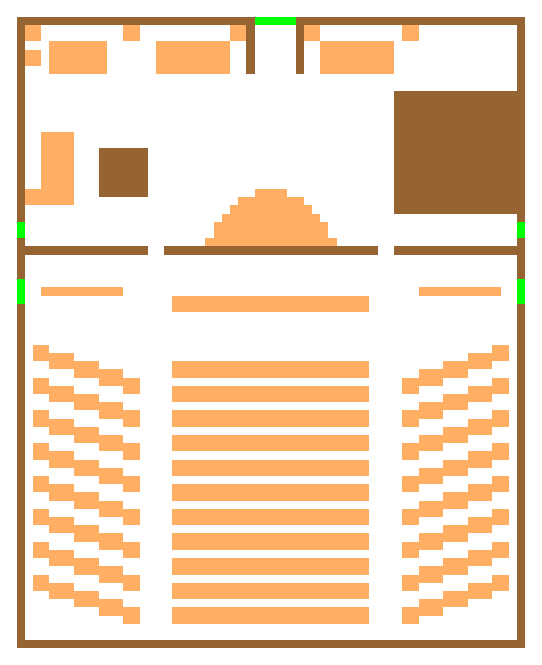
\includegraphics[width=0.3\textwidth]{figures/D.eps}
    \caption{D wing.}
    \label{fig:dwing}
\end{figure}

\begin{figure}
    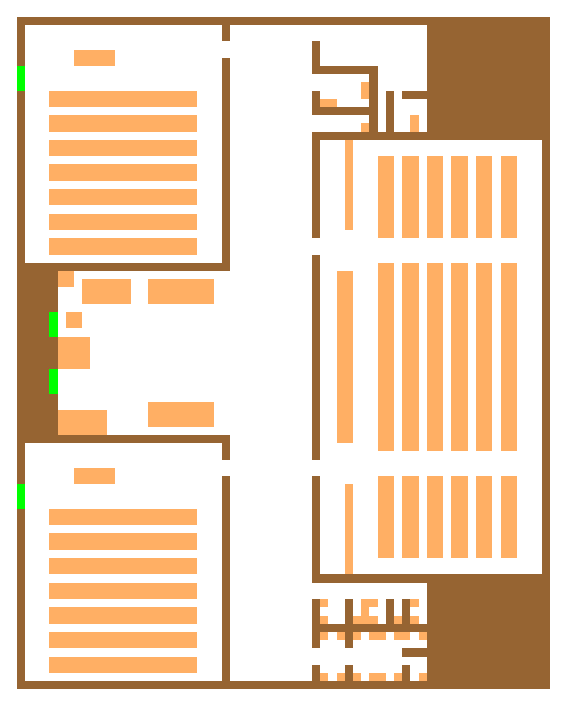
\includegraphics[width=0.3\textwidth]{figures/E.eps}
    \caption{E wing.}
    \label{fig:ewing}
\end{figure}

For each object (wall, table, vending machine etc.) we estimate error in either
of its dimensions to be +-0.2 meters (half of the length of one cell side).
Using $PI$ cell states we specified primary positions for individuals
(students) - students primarily occupy seats in lecture rooms, some may be in
the halls - which simulates a common study session.
For each of the wings we created five different scenarios that describe
various building configurations, from normal state to the case where some of
the exits or even room entrances are blocked/closed.

In each experiment we compute a total evacuation time: a time interval between
alarm going off and an extraction of the last individual.
We are also interested in the time each individual was exposed to the smoke;
in each experiment we report a maximum value.
We are interested if this value will not exceed a threshold of 5 minutes.
With the purpose of obtaining acceptable statistical data, the final results are
obtained by averaging results of 10000 independent replications of each
experiment.

\subsection{Description of buildings}
A ground floor of the D section consists of a lecture room D105 with capacity of
300 and a vestibule that is approximately half the size of the lecture room;
there are two narrow entrances into the lecture room from the entrance hall;
there are a total of five exits from the building: primary one on the east
side, a pair of exits on the north/south side of the vestibule and a similar
pair inside the lecture room.
Note that a south vestibule exit leads to the corridor between D and A segments
where an actual exit is located.

A ground floor of the E section consists of a lecture room E112 with capacity of
156, two smaller lecture rooms E104 \& E105 of capacity 72 each, several toilets,
a maintenance room and a corridor in between;
there are two narrow entrances into the E112 and one entrance into E104 and
E105 each;
there are a total of four exits, each situated on the east side of the building:
two from the hall in the middle and two from inside E104 and E105 lecture rooms.
There is also a corridor linking E and C segments where another exit is
situated, but it is too far away and requires blocking of all four E exits in
order to be used; since it is not even considered in evacuation plans, C section
was completely ommitted.

\subsection{Experiments}
In all of the cases we consider a number of individuals to be 350 (full
attendance + someone in the halls) and one random source of fire. For each wing
we will consider several fire scenarios that mostly differ by an availiability
of selected exits, i.e. some exits or doors are made locked.

These cases are not as unrealistic as they seem, e.g. side exits from inside D105 are
usually locked and are unlocked automatically when emergency occurs.
In case a fire causes (or was caused by) a wiring fault, there is a probability
that the doors might remain locked.
Furthemore, these exits are always covered by external mechanical window blinds,
which undoubtfully slows evacuation down.
The exact same argument applies to exits from within E104 and E105 lecture
rooms.
Next, during our study we witnessed several cases when one of the entrances
to D105 or E112 was locked for no apparent reason and a handyman had had to fix
it.
The last argument might sound strange, but the fact is, most of the students we
interviewed did not even know that there are exits from E104 and E105 lecture rooms.
During emergency, a group effect may take place and even those who know about
the existence of these exits might panic and forget about them while following
the majority that heads to the corridors.

Here is a list of five scenarios we will be considering for D wing:

\begin{itemize}
    \item D1: a normal state
    \item D2: one exit in D105 and one side exit in the entrance hall are
    blocked
    \item D3: exits from inside D105 are blocked
    \item D4: all four side exits are blocked
    \item D5: all side exits are blocked, one of D105 entrances is blocked
    (worst-case scenario)
\end{itemize}

Bitmaps for each of the cases can be found in \texttt{experiments} folder.
Results for each case reporting total evacuation time and a maximum smoke
exposure time are displayed in Table \ref{table:results_d}.

\begin{center}
    \captionof{table}{TODO}
    \label{table:results_d}
    \begin{tabular}{ c | c | c | c | c | c | c | c }
        \hline
        Case & D1 & D2 & D3 & D4 & D5 & D5-3 & D5-4 \\
        \hline
        Evacuation time (seconds) & 0 & 0 & 0 & 0 & 0 & 0 & 0 \\
        Maximum exposure (seconds) & 0 & 0 & 0 & 0 & 0 & 0 & 0 \\
        \hline
    \end{tabular}
\end{center}

Before evaluating building plans, let us first inspect the results to see if
they make sense.
In D1 all exits were functional and those sitting in D105 used two closest ones,
which is what one would expect to happen.
Those exits are not very far and an extraction time of forty seconds looks
reasonable.
In D2 one of side exits from inside the lecture room was blocked, the one
outside was free, but it took quite longer to evacuate because of the
narrow door in the way.
In D3 the same happens on the other side, which again makes evacuation even
longer.
In D4 only main entrance is preserved, but evacuation time is roughly the same;
the reason for this is that, in both D3 and D4 cases, large queues had been
created at the narrow exits from the lecture room
(see Figure~\ref{fig:d4bn}), which is the main source of delay.
In D5 one of this entrances is blocked and the effect here is even more
apparent, see Figure~\ref{fig:d5bn}.
This event is known as \emph{bottleneck effect}.

\begin{figure}
    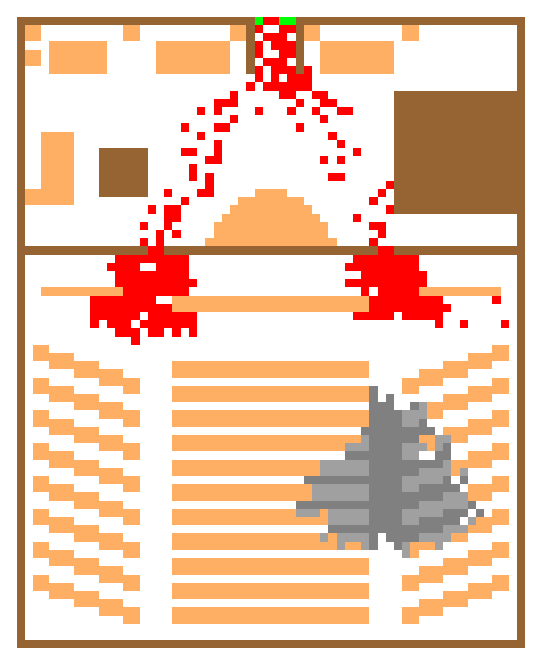
\includegraphics[width=0.3\textwidth]{figures/d4bn.eps}
    \caption{D4: individuals accumulate at narrow doors.}
    \label{fig:d4bn}
\end{figure}

\begin{figure}
    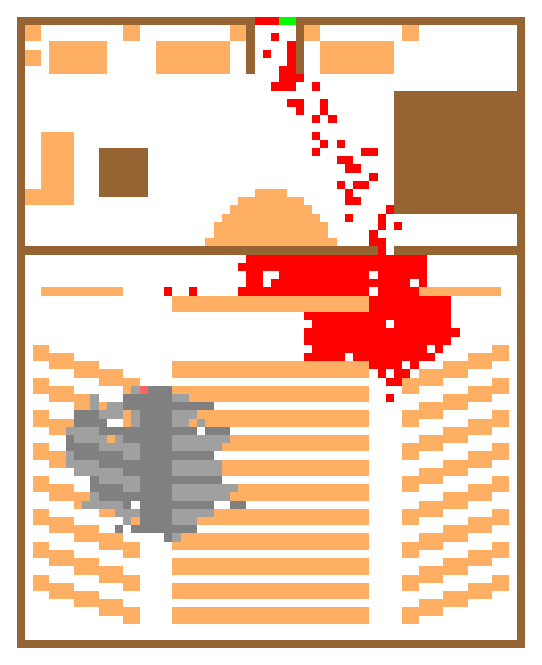
\includegraphics[width=0.3\textwidth]{figures/d5bn.eps}
    \caption{D5: blocking one of the doors results in disasterous effect.}
    \label{fig:d5bn}
\end{figure}

Lecture room entrances seem to be a critical point; to confirm this, let's
increase the door width and see what will be the impact.
We use modifications of D5 case and vary door width from 2(D5) to 3 (D5-3)
and 4 (D5-4).
Results are displayed in the table \ref{table:results_d}.

It is clear that enlarging entrance(s) width will result in significantly more
successful evacuation.
Note that this should not necessarily mean that occupants must break down walls;
a door to D105 room has a (re-)movable part that is usually held fixed and
occupants should not forget about it.

Let us now consider E wing. These are scenarios:
\begin{itemize}
    \item E1: a normal state
    \item E2: E104 exit is blocked
    \item E3: both E104 and E105 exits are blocked
    \item E4: both E104 and E105 exits are blocked, one of the main exits is
    blocked
    \item E5: both E104 and E105 exits are blocked, one of the main exits is
    blocked, one of E112 entrances is blocked (worst-case scenario)
\end{itemize}

The results are reported in Table \ref{table:results_e}.
Again, as we gradually block majority of exits, we inspect similar behaviour and
results.

\begin{center}
    \captionof{table}{TODO}
    \label{table:results_e}
    \begin{tabular}{ c | c | c | c | c | c }
        \hline
        Case & E1 & E2 & E3 & E4 & E5 \\
        \hline
        Evacuation time (seconds) & 0 & 0 & 0 & 0 & 0 \\
        Maximum exposure (seconds) & 0 & 0 & 0 & 0 & 0 \\
        \hline
    \end{tabular}
\end{center}

In the final experiment suite, we explore worst-case scenarios (D5 and E5) in
more detail by varying a number of occupants from 200 to 500 and then varying
a number of fire sources from 1 to 3.
The results are displayed separately for D (Table~\ref{table:results_d5})
and E (Table~\ref{table:results_e5}) wings.
Again, we report a total evacuation time (e) and a smoke exposure time (s),
both in seconds.

\begin{center}
    \captionof{table}{TODO}
    \label{table:results_d5}
    \begin{tabular}{ c | c | c | c | c }
        \hline
        Occupants & 200 & 300 & 400 & 500 \\
        1 smoke source(e) & 0 & 0 & 0 & 0 \\
        (s) & 0 & 0 & 0 & 0 \\
        2 smoke sources(e) & 0 & 0 & 0 & 0 \\
        (s) & 0 & 0 & 0 & 0 \\
        3 smoke sources(e) & 0 & 0 & 0 & 0 \\
        (s) & 0 & 0 & 0 & 0 \\
        \hline
    \end{tabular}
\end{center}


\begin{center}
    \captionof{table}{TODO}
    \label{table:results_e5}
    \begin{tabular}{ c | c | c | c | c }
        \hline
        Occupants & 200 & 300 & 400 & 500 \\
        1 smoke source(e) & 0 & 0 & 0 & 0 \\
        (s) & 0 & 0 & 0 & 0 \\
        2 smoke sources(e) & 0 & 0 & 0 & 0 \\
        (s) & 0 & 0 & 0 & 0 \\
        3 smoke sources(e) & 0 & 0 & 0 & 0 \\
        (s) & 0 & 0 & 0 & 0 \\
        \hline
    \end{tabular}
\end{center}

It is clear that increasing a number of individuals will increase both
evacuation time and smoke exposure; increasing number of smoke sources, however,
will only increase the latter.
Nonetheless, in all of our experiments smoke exposure rates are way below the
threshold, which indicates that even in the worst case no one should suffer
substantial damage.
Therefore, we declare both D and E wings to be suitable for emergency
evacuations.

\section{Conclusion}
In this project we considered a suitability of D and E wings of a FIT VUT campus
for emergency evacuations due to the threat of fire.
Inspired by research by Tissera et al.~\cite{Tissera1, Tissera2} and
Yuan et al.~\cite{Yuan} and, exploiting concepts of fire and smoke spreading and
crowd dynamics, we designed a model of these complex phenomena based on
cellular automata.
We then designed a diverse experiment suite representing different fire
scenarios.
Evaluating these cases we collected various statistics that allowed us to
declare that both building of interest are indeed suitable for emergency
evacuations.
